\documentclass[a0,landscape]{a0poster}

\usepackage{fontspec}
%\defaultfontfeatures{Ligatures=TeX}
\setmainfont{Fira Sans}
%\setmonofont{Fira Mono}

\renewcommand{\familydefault}{\sfdefault}

\usepackage{multicol}
\columnsep=100pt
\columnseprule=3pt

\usepackage[svgnames]{xcolor}

\usepackage{graphicx}

\graphicspath{{images/}}

\usepackage{booktabs}

\usepackage[font=small,labelfont=bf]{caption}

\usepackage{amsfonts, amsmath, amsthm, amssymb}
\usepackage{wrapfig}

\usepackage{url}

\setlength\parindent{0pt}

\usepackage{array}

\usepackage{tcolorbox}

\begin{document}

\begin{minipage}[b][8cm][c]{0.6\textwidth}
{\VeryHuge
 \color{NavyBlue}
 \textbf{Kelompok Keahlian Material Fungsional Maju}\\
}
\color{Blue}
{\Huge Program Studi Teknik Fisika, Fakultas Teknologi Industri}\\
{\Huge Institut Teknologi Bandung}
\end{minipage}
%
\begin{minipage}[b][8cm][c]{0.5\textwidth}

\includegraphics[width=8cm]{ITB_logo.pdf}\\
\end{minipage}

\vspace{1cm}

\Large

\begin{multicols}{3}

\begin{tcolorbox}[
  colback=blue!5,
  colframe=green!40!black,
  title=Anggota]
{\centering
\begin{tabular}{
|>{\centering\arraybackslash}m{8cm}
|>{\centering\arraybackslash}m{25cm}|}
%\begin{tabular}{cc}
\hline
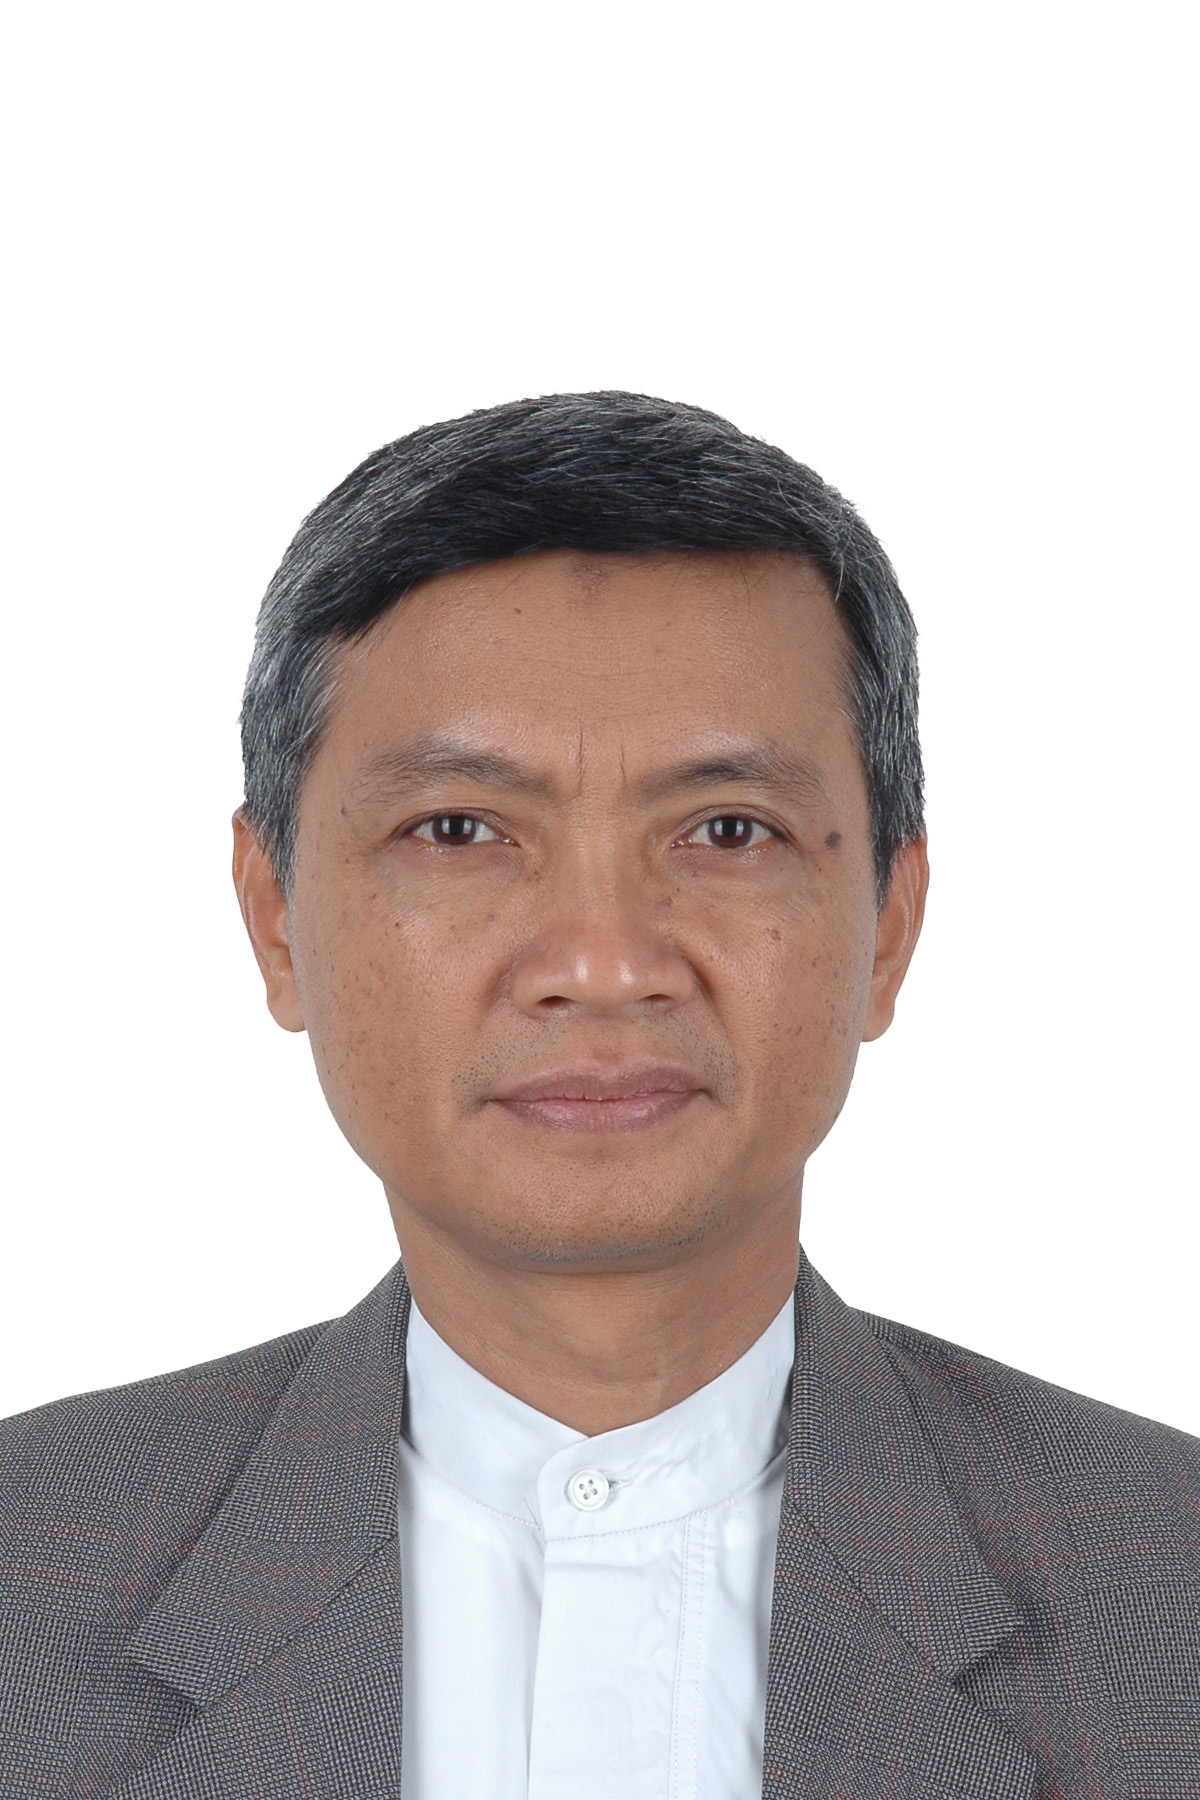
\includegraphics[height=7cm]{HermawanKDipojono.png} &
Prof. Ir. Hermawan K. Dipojono. MSEE, PhD  \\
\hline
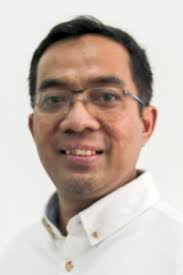
\includegraphics[height=7cm]{BrianYuliarto.png} &
Prof. Brian Yuliarto \\
\hline
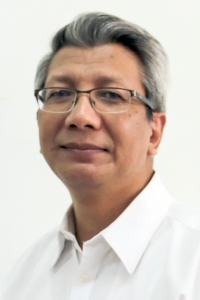
\includegraphics[height=7cm]{AhmadNuruddin.png} &
Dr. Ahmad Nuruddin \\
\hline
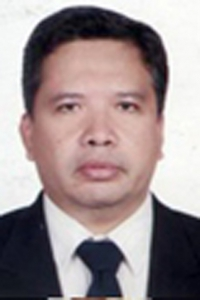
\includegraphics[height=7cm]{Nugraha.png} &
Dr. Nugraha \\
\hline
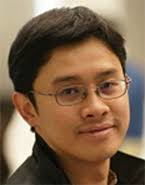
\includegraphics[height=7cm]{KemalAgusta.png} &
Dr. Mohammad Kemal Agusta \\
\hline
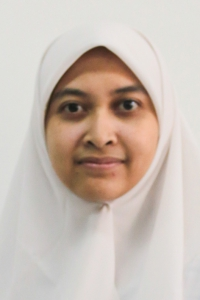
\includegraphics[height=7cm]{DamarRastriAdhika.png} &
Dr. Damar Rastri Adhika \\
\hline
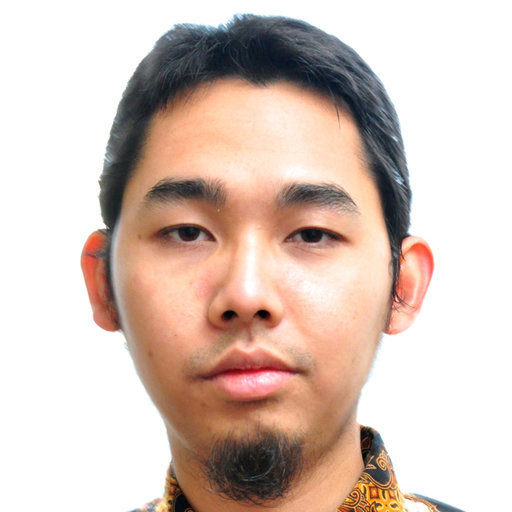
\includegraphics[height=7cm]{AdhityaGandaryusSaputro.png} &
Dr. Adhitya Gandaryus Saputro \\
\hline
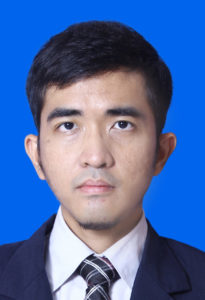
\includegraphics[height=7cm]{FadjarFathurrahman.png} &
Dr. Fadjar Fathurrahman \\
\hline
\end{tabular}
\par
}
\end{tcolorbox}

{\LARGE
\begin{tcolorbox}[
  colback=blue!5,
  colframe=blue!40!black,
  title=Visi]
\vspace{1cm}
Menjadi kelompok keahlian berkelas dunia yang memiliki keunggulan
dalam aspek keilmuan material fungsional maju
\end{tcolorbox}
}
%
{\LARGE
\begin{tcolorbox}[
  colback=blue!5,
  colframe=blue!40!black,
  title=Misi]
\vspace{1cm}
\begin{itemize}
\item Mendukung ITB dalam penyelenggaraan pendidikan, penelitian, dan pengabdian 
 masyarakat di bidang ilmu kerekayasaan material fungsional maju.
\item Mengembangkan keilmuan dan keahlian, serta berkontribusi dalam menyelesaikan
 permasalahan kerekayasaan masyarakat, industri, dan pemerintah yang membutuhkan solusi berupa material fungsional maju.
\item Menjalin sinergi dan kerjasama keilmuan dan profesi di bidang yang terkait.
\end{itemize}
\end{tcolorbox}
}
%
{\LARGE
\begin{tcolorbox}[
  colback=blue!5,
  colframe=blue!40!black,
  title=Tujuan]
\vspace{1cm}
\begin{itemize}
\item Berkontribusi dalam \textit{state of the art} pengembangan fundamental sains material fungsional maju sebagai komponen utama penyokong keilmuan Teknik Fisika
\item Pengembangan keahlian dalam rangka menawarkan solusi kerekayasaan pada berbagai permasalahan kerekayasaan di masyarakat baik industri maupun pemerintah.
\end{itemize}
\end{tcolorbox}
} 
%
{\LARGE
\begin{tcolorbox}[
  colback=blue!5,
  colframe=blue!40!black,
  title=Peta Jalan Penelitian]
\vspace{1cm}
Topik-topik riset dipilih berdasarkan kondisi terkini di
garis depan keilmuan serta pertimbangan jangka panjang dari kebutuhan masyarakat 
Indonesia, dengan juga mempertimbangkan keberlanjutan penelitian dari anggota selama 
beberapa tahun terakhir. Untuk 5 – 10 tahun ke depan. Topik-topik tersebut dibagi menjadi 
dua sub-kajian yaitu:
\begin{itemize}
\item Sintesis dan Rekayasa permukaan material nano
\item Komputasi multiskala pada sistem permukaan/antarmuka
\end{itemize}
\end{tcolorbox}
} 

{\LARGE
\begin{tcolorbox}[
  colback=blue!5,
  colframe=blue!40!black,
  title=Sintesis dan Rekayasa permukaan material nano]
\vspace{1cm}
Sub-kajian ini bertujuan untuk melakukan pengembangan,
penerapan metode sintesis dan rekayasa 
struktur, morfologi, dan permukaan material nano untuk menghasilkan material fungsional 
yang sifatnya dapat diatur sesuai dengan aplikasi yang diinginkan.

Fokus pengembangan pada sub kajian ini terbagi menjadi dua bagian: (1) teknik sintesis dan 
rekayasa struktur material nano untuk aplikasi energi, lingkungan, kesehatan, dan pangan, 
(2) metode karakterisasi material nano dan pengujian kinerja material sebagai material 
aktif dalam aplikasi energi, lingkungan, kesehatan, dan pangan.

Anggota KK yang akan secara khusus terlibat dalam sub-kajian ini adalah: (1) Dr. Brian 
Yuliarto, (2) Dr. Ahmad Nuruddin, (3) Dr. Nugraha, dan (5) Dr. Damar Rastri Adhika.
\end{tcolorbox}
}

{\LARGE
\begin{tcolorbox}[
  colback=blue!5,
  colframe=blue!40!black,
  title=Komputasi multiskala pada sistem permukaan/antarmuka]
\vspace{1cm}
Sub-kajian ini bertujuan untuk melakukan pengembangan dan penerapan dari metode komputasi dalam mempelajari fenomena-fenomena fisis yang terjadi pada sistem permukaan dan antarmuka seperti perancangan berbagai material katalis yang aplikasinya yang relevan dengan kebutuhan teknologi energi, serta perancangan advanced material untuk aplikasi sensor gas dan biomolekul. Prinsip kerja dari teknologi tersebut dapat dideskripsikan secara fundamental sebagai interaksi antara molekul dengan permukaan/antarmuka dari suatu material. 

Anggota KK yang akan secara khusus terlibat dalam sub-kajian ini adalah: (1) Prof. Dr. Hermawan K. Dipojono, (2) Dr. Mohammad Kemal Agusta, (3) Dr. Adhitya Gandaryus Saputro dan (4) Dr. Fadjar Fathurrahman.
\end{tcolorbox}
}


\end{multicols}


\end{document}
